\documentclass[conference]{IEEEtran}
\IEEEoverridecommandlockouts

\usepackage[T1]{fontenc}
\usepackage[utf8]{inputenc}
\usepackage{cite}
\usepackage{amsmath,amssymb,amsfonts}
\usepackage{algorithmic}
\usepackage{graphicx}
\usepackage{textcomp}
\usepackage{xcolor}
\usepackage{booktabs}
\usepackage{tabularx}
\usepackage{enumitem}
\usepackage{url}
\usepackage[hidelinks]{hyperref}
\hypersetup{
  pdfauthor={},
  pdftitle={Authority-Aligned Linearization for Rescue-Service Incident Response over Intermittent Edge Networks},
  pdfsubject={NCA 2026 Submission},
  pdfkeywords={},
  pdfproducer={},
  pdfcreator={}
}
\usepackage[nameinlink,noabbrev]{cleveref}
\usepackage{tikz}
\usetikzlibrary{positioning,arrows.meta,shapes.geometric,fit,backgrounds}

\setlist[itemize]{leftmargin=*,topsep=2pt,itemsep=2pt}
\setlist[enumerate]{leftmargin=*,topsep=2pt,itemsep=2pt}

\newcommand{\systemname}{Tiered Sync Architecture}

\title{Offline-First Incident Information: A Tiered Sync Architecture for Rescue Service Operations over Intermittent Mesh Networks}

\author{\IEEEauthorblockN{Anonymous Author(s)}
\IEEEauthorblockA{Anonymous Affiliation\\
Submitted to NCA 2026 (double-blind review)}}

\begin{document}

\maketitle

\begin{abstract}
In rescue-service incident response, one principal holds operational command authority at every moment. At the same time, responders must keep working through responder and backhaul partitions. Authority-bearing incident decisions must therefore stay attributable to that single commander under intermittent connectivity, where the standard distributed-systems toolkit does not fit well. Consensus over-serves a workload that is mostly lookups plus append-only reporting. Conflict-free replicated data type (CRDT) merge is mergeable-by-default, so it cannot encode authority for non-commutative decisions. Local-first systems optimize a replica autonomy that this domain rejects. We present \methodname{} (AAL), a consistency discipline for this setting. AAL places the incident-journal linearization point at the edge node that currently holds command authority. Non-authority data (reference state, field submissions, materialized views) stays locally available and is forwarded eventually, and command transfer uses fenced promotion, not leader election. TLA+ and Hypothesis models check the single-authority and fenced-promotion invariants, and a Docker Compose prototype measures field-submission propagation, wide-area recovery, throughput, duplicate replay, and stale-epoch rejection. As a result, partitions on either responder or backhaul links do not block command-edge progress, and stale-epoch traffic cannot poison the incident journal. Because the fence rejects stale traffic before the journal write, that rejection costs 2.5$\times$ less than a successful commit. The cost is no automatic failover; promotion is operator-initiated.

\end{abstract}

\begin{IEEEkeywords}
offline-first systems, edge computing, distributed systems, single-writer replication, intermittent connectivity, mesh networks, prototype evaluation
\end{IEEEkeywords}

\section{Introduction}

Edge applications increasingly span devices that do not share a continuously connected network. Vehicle-mounted compute nodes, field tablets, and regional services may alternate between full connectivity, mesh-only connectivity, and total isolation. Public-safety mesh measurements show that such partitions can be frequent rather than exceptional in forested operational terrain \cite{zimbelman2022mesh}, while broader emergency-communications surveys describe heterogeneous LTE, ad hoc, and mission-critical network conditions \cite{kumbhar2015legacy,hoyhtya2018critical,wang2023overview}. A useful edge architecture must therefore specify not only how data moves when links are present, but also which writes remain meaningful when links are absent.

The dominant replication patterns make different trade-offs. Consensus-based state-machine replication, including Paxos- and Raft-style protocols, provides a single ordered log when a quorum is available \cite{lamport1998parttime,ongaro2014raft}. Multi-primary replication maximizes local write availability but pushes conflict resolution into reconciliation after partitions \cite{mucha2023database}. CRDT and local-first systems preserve availability for data types whose updates can be merged without coordination \cite{kleppmann2019localfirst,almeida2014delta}. These patterns are powerful, but they do not directly capture a class of edge applications in which events are authority-bearing: an event is not merely a state update, but an ordered decision made by a designated operational principal.

This paper uses incident-information management as a concrete instance of that problem. In command-hierarchical emergency response, some field observations can be queued locally, but authoritative incident state must be sequenced by the current command role. A wrong merge can be worse than a delayed commit if it produces inconsistent resource assignments, status transitions, or hazard annotations. The application domain motivates the design, but the systems question is broader: how should authority-bearing data be synchronized across intermittently connected edge tiers?

The contribution is a tiered synchronization architecture for authority-bearing data over intermittent multi-tier connectivity. The architecture combines a single-writer incident journal at the command vehicle, durable forward-only outboxes at responder vehicles and tablets, and explicit manual promotion rather than automatic leader election. It is structurally related to shared-log systems such as Tango \cite{balakrishnan2013tango}, but differs in why the writer exists: the writer is an operational authority selected by the incident workflow, not merely an elected replica leader. The submission version is being migrated toward an NCA evaluation that will add safety verification and baseline comparison results.

The rest of the paper is organized as follows. \Cref{sec:related} positions the design against state-machine replication, local-first systems, and edge-connectivity work. \Cref{sec:architecture} presents the three-tier architecture and fault model. \Cref{sec:sync} specifies the synchronization protocol. \Cref{sec:implementation} summarizes the prototype scaffold. \Cref{sec:validation} marks the planned NCA evaluation and remaining measurement work.

\section{Background and Related Work}
\label{sec:related}

\subsection{Replication and State-Machine Replication}

The obvious baseline for a single ordered incident journal is state-machine replication. Paxos established the consensus foundation for replicated logs in asynchronous systems with failures \cite{lamport1998parttime}, and Raft made the single-leader log model easier to understand and implement \cite{ongaro2014raft}. More recent systems explore other points in the linearizable-replication design space, including broadcast-based replication in Hermes \cite{katsarakis2020hermes}, predictable performance in HoliPaxos \cite{liang2025holipaxos}, and replicated-key linearizability in LARK \cite{gooding2025lark}. Tango is especially relevant because it builds distributed data structures over a shared log and then materializes application views from that log \cite{balakrishnan2013tango}.

The Rescue OIS incident journal follows the shared-log/materialized-state pattern, but its writer is not chosen by a consensus protocol. The writer is the command vehicle designated by the operational workflow. That choice intentionally trades automatic write failover for an authority model that is explainable to operators and auditable after the incident. \Cref{sec:validation} will compare this design against a Raft baseline in the next phase of the NCA submission work.

\subsection{Local-First and CRDT-Based Replication}

Local-first systems prioritize local availability, user control, and continued operation under poor connectivity \cite{kleppmann2019localfirst}. Much of that work relies on coordination-free replication or CRDT-based synchronization, including efficient delta-based variants \cite{almeida2014delta}. Recent work focuses on preserving application-level invariants and verifying safety properties in replicated settings \cite{haas2023lore,kohler2025consistent,jannes2021owebsync}. Disconnected-operation database replication takes a related multi-primary position: continue local work and reconcile when connectivity returns \cite{mucha2023database}.

Those techniques are valuable for naturally mergeable state, but the incident journal contains ordered, authority-bearing events. CRDTs would still require application-specific semantics for conflicting command decisions, resource assignments, or status transitions. The architecture in this paper therefore adopts offline-first availability for reads and queued submissions, while keeping authoritative incident commits under one command-side sequencer.

\subsection{Edge Computing and Intermittent Connectivity}

Public-safety communications research spans legacy narrowband systems, LTE and 5G public-safety services, ad hoc and vehicular networking, and rapidly deployable mesh-style infrastructure \cite{kumbhar2015legacy,hoyhtya2018critical,wang2023overview}. The most directly relevant field evidence comes from public-safety mesh-radio measurements in forested terrain, where full network connectivity was present only about a third of the observation time and vegetation was the dominant predictor of disconnection \cite{zimbelman2022mesh}. Offline crisis-mapping prototypes such as CRIMP similarly treat vehicles as opportunistic carriers between fragmented field networks \cite{paul2019crimp}.

These works motivate a partition-frequent fault model, but they do not prescribe the application-level consistency model for authority-bearing incident state. The architectural contribution here is above the transport layer: the mesh is treated as intermittent transit, while sequencing, idempotency, promotion, and reconciliation remain explicit protocol concerns.

\section{System Architecture}
\label{sec:architecture}

\subsection{Operational Setting and Requirements}
\label{sec:requirements}

The deployment environment is municipal rescue-service incident response in a country with substantial unpopulated forested terrain. Incidents are managed by a small set of vehicles, typically two to ten per incident, operating up to several hours away from the regional dispatch centre. Each vehicle is staffed by personnel using rugged tablets to view and update operational information. The incident is led by a designated command vehicle whose role is operationally fixed at dispatch and reassigned only by explicit operator decision. The publicly available rescue-service guidance summarised in Section~\ref{sec:introduction} establishes that incident-planning information must be available without continuous connectivity, that secrecy-protected and non-secret material must be handled with different operational discipline, and that incident plans are layered, ongoing operational artefacts rather than static documents~\cite{rsg-rad201, rsg-kommunalplan}.

We distinguish externally motivated requirements from design assumptions and deployment constraints. The distinction matters because an operational command authority does not logically require a single-writer storage design; aligning the storage authority boundary with the operational authority boundary is the design choice made in this paper.

\begin{itemize}
  \item \textbf{R1 (Offline operation).} Each tier must continue functioning on previously synchronised data without connectivity to any other tier.
  \item \textbf{R2 (Durable forward-only submission).} Field observations entered on tablets must never be lost, including across vehicle restart and prolonged partition.
  \item \textbf{R3 (Attributable command authority).} Decisions on resource assignments, status transitions, and hazard annotations must be attributable to a single operationally designated authority at every instant of the incident.
  \item \textbf{R4 (Predictable network behaviour).} The wireless mesh substrate must not cause cascading failures (broadcast storms, routing loops) when nodes join, leave, or partition.
  \item \textbf{R5 (No parallel identity).} Authentication, authorisation, and audit must reuse the rescue-service organisation's existing certificate authority and identity provider; no parallel identity stack may be introduced.
\end{itemize}

\begin{table}[t]
\centering
\caption{Traceability from adopted constraints to architectural consequences.}
\label{tab:req-trace}
\footnotesize
\begin{tabularx}{\columnwidth}{@{}l l X@{}}
\toprule
\textbf{Item} & \textbf{Type} & \textbf{Result} \\
\midrule
Offline operation & Operational requirement & Edge cache and local services. \\
Durable field submission & System requirement & Tablet/edge outbox and retry. \\
Attributable command authority & Operational assumption & Single command-side journal writer. \\
Predictable network behavior & Deployment constraint & Mesh as routed transit; no stretched user VLAN. \\
Existing identity integration & Integration constraint & mTLS/CA integration and mapped identities. \\
\bottomrule
\end{tabularx}
\end{table}

The five design principles in Section~\ref{sec:principles} are derived from this traceability rather than asserted independently. The mapping is explicit: \textit{offline-first} from R1; \textit{single incident writer} from R3 and the chosen storage-authority boundary; \textit{forward-only edits} from R2 directly and R3 indirectly; \textit{mesh as transit only} from R4 directly and R5 indirectly, because stretched VLANs would extend the trust surface across the mesh; \textit{existing identity} from R5.

\subsection{Design Principles}
\label{sec:principles}

The system is built around five principles:
\begin{itemize}
  \item \textbf{Offline-first} (R1): all previously synchronised data remains available without connectivity.
  \item \textbf{Single incident writer} (R3, R2): exactly one command node sequences and commits incident events.
  \item \textbf{Forward-only edits} (R2, R3): tablets and responder vehicles enqueue edits locally and forward them upstream.
  \item \textbf{Mesh as transit only} (R4, R5): the wireless mesh carries traffic between edge nodes, but does not expose user VLANs end to end.
  \item \textbf{Existing identity} (R5): the deployment integrates with the authority's established identity and certificate infrastructure.
\end{itemize}

\subsection{Tier 1: Regional Core}

The regional core hosts the authoritative master-data platform in the target deployment. It uses a spatial database, a publication pipeline that stages, validates, and promotes geodata into versioned offline packages, and a tile-serving stack for map data. A reverse proxy terminates TLS and routes API traffic to internal services. A VPN overlay connects enrolled vehicles when WAN is present. Published packages consist of map bundles, compressed attachment archives, and SHA-256 manifests that edge nodes can pull over HTTP range requests. Section~\ref{sec:implementation} separates which of these elements are implemented and which are deployment scaffolding.

\subsection{Tier 2: Vehicle Edge}

The vehicle edge tier is the architectural center of the paper. Each vehicle carries the same edge hardware profile, but nodes operate in one of two software roles:
\begin{itemize}
  \item \textbf{Command vehicle:} commits incident events, assigns sequence numbers, materializes incident state, and backhauls to core when WAN is present.
  \item \textbf{Responder vehicle:} caches master data, serves local tablets, and queues field edits in an outbox until they can be forwarded to command.
\end{itemize}

This role split is intentional. It preserves hardware interchangeability while keeping the incident journal under one authority-bearing node at any time. Any responder can be promoted to command by configuration and operational procedure.

\subsection{Tier 3: Field Tablets}

Field tablets are leaf clients attached to a local vehicle only. They use an encrypted local database and local tile cache, and they communicate over HTTPS with the edge node in their vehicle. Tablets have no direct mesh participation and no direct internet dependency. This sharply limits the exposed trust and connectivity surface.

\subsection{State Classes and Consistency Contracts}
\label{sec:state-taxonomy}

The single-writer constraint applies to authority-bearing incident-journal entries, not to every byte in the system. Figure~\ref{fig:state-contracts} separates the main state classes and the contract each one uses.

\begin{figure}[t]
\centering
% \begin{tikzpicture}[
%   x=1cm,y=1cm,
%   every node/.style={font=\scriptsize},
%   head/.style={draw, fill=gray!25, font=\scriptsize\bfseries, align=center, minimum height=0.42cm, inner sep=1pt},
%   state/.style={draw, fill=gray!10, align=left, text width=1.75cm, minimum height=0.48cm, inner sep=2pt},
%   src/.style={draw, align=center, text width=1.55cm, minimum height=0.48cm, inner sep=2pt},
%   contract/.style={draw, align=left, text width=4.25cm, minimum height=0.48cm, inner sep=2pt},
%   emph/.style={contract, double, double distance=0.5pt}
% ]
% \node[head, text width=1.75cm] at (0.90,0) {State};
% \node[head, text width=1.55cm] at (2.65,0) {Authority / source};
% \node[head, text width=4.25cm] at (5.60,0) {Synchronization contract};

% \node[state] at (0.90,-0.55) {Reference data};
% \node[src] at (2.65,-0.55) {regional core};
% \node[contract] at (5.60,-0.55) {one-way core-to-edge replication; eventual convergence};

% \node[state] at (0.90,-1.15) {Immutable artifacts};
% \node[src] at (2.65,-1.15) {publisher / core};
% \node[contract] at (5.60,-1.15) {manifest/package/hash validation where implemented};

% \node[state] at (0.90,-1.75) {Field observations};
% \node[src] at (2.65,-1.75) {tablet / responder};
% \node[contract] at (5.60,-1.75) {locally durable outbox; at-least-once forwarding; idempotent accept};

% \node[state] at (0.90,-2.35) {Command decisions};
% \node[src] at (2.65,-2.35) {command edge};
% \node[emph] at (5.60,-2.35) {single-writer applies only here; total order by event\_seq};

% \node[state] at (0.90,-2.95) {Materialized state};
% \node[src] at (2.65,-2.95) {journal};
% \node[contract] at (5.60,-2.95) {derived/rebuildable; not authoritative};

% \node[state] at (0.90,-3.55) {Audit events};
% \node[src] at (2.65,-3.55) {edge / core};
% \node[contract] at (5.60,-3.55) {eventual forwarding; validation incomplete};
% \end{tikzpicture}
\scriptsize
\setlength{\tabcolsep}{3pt}
\begin{tabularx}{\columnwidth}{@{}p{0.24\columnwidth}p{0.20\columnwidth}X@{}}
\toprule
\textbf{State} & \textbf{Authority/source} & \textbf{Synchronization contract} \\
\midrule
Reference data & regional core & One-way core-to-edge replication; eventual convergence. \\
Immutable artifacts & publisher / core & Manifest, package, or hash validation where implemented. \\
Field observations & tablet / responder & Locally durable outbox; at-least-once forwarding; idempotent accept. \\
Command decisions & command edge & Single-writer rule applies only here; total order by \textit{event\_seq}. \\
Materialized state & journal & Derived and rebuildable; not authoritative. \\
Audit events & edge / core & Eventual forwarding; validation incomplete. \\
\bottomrule
\end{tabularx}
\caption{State classes use different synchronization contracts. The single command writer applies to authority-bearing journal entries, not to every object in the system; materialized state is derived, and audit forwarding validation remains incomplete.}
\label{fig:state-contracts}
\end{figure}

\subsection{Network Segmentation}

Each vehicle is intended to carry a router enforcing a five-VLAN segmentation model keyed on a per-vehicle identifier. Tablets reach only the local \texttt{ops-api} endpoint over HTTPS, user VLANs are not extended across the mesh, and the mesh operates as Layer~3 transit for application-layer traffic between edge nodes. Figure~\ref{fig:topology-scope} separates this target deployment from the narrower Docker/Python path measured in Section~\ref{sec:validation}.

\begin{figure}[t]
\centering
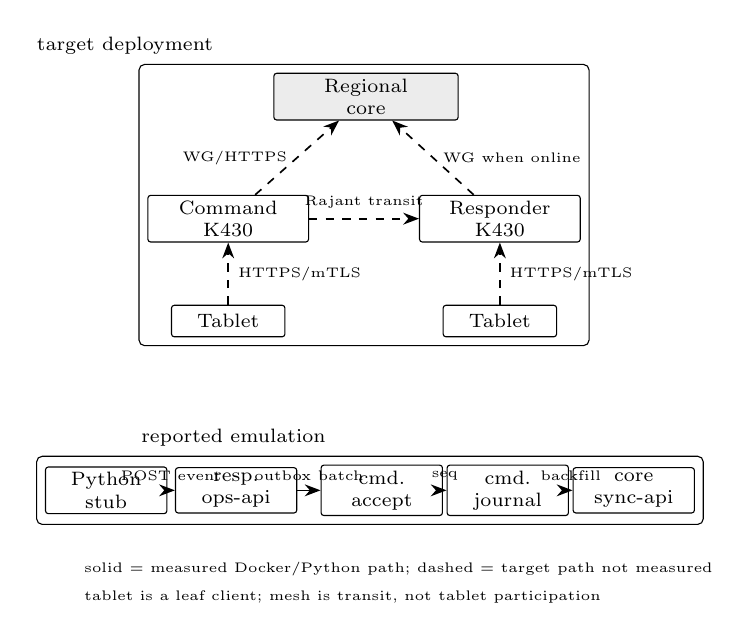
\begin{tikzpicture}[
  node distance=4mm,
  every node/.style={font=\scriptsize},
  svc/.style={draw, rounded corners=1pt, align=center, minimum height=5mm, inner sep=2pt},
  core/.style={svc, fill=gray!15, text width=22mm},
  edge/.style={svc, text width=19mm},
  tablet/.style={svc, text width=13mm, minimum height=4mm},
  emu/.style={svc, fill=white, text width=16mm, minimum height=5mm},
  targetlink/.style={->, >=Stealth, dashed, semithick},
  measuredlink/.style={->, >=Stealth, semithick},
  boundary/.style={draw, rounded corners=2pt, inner sep=3pt}
]
\node[core] (core) at (3.75,1.0) {Regional\\core};
\node[edge] (cmd) at (2.0,-0.55) {Command\\K430};
\node[edge] (resp) at (5.45,-0.55) {Responder\\K430};
\node[tablet] (tab1) at (2.0,-1.85) {Tablet};
\node[tablet] (tab2) at (5.45,-1.85) {Tablet};

\draw[targetlink] (tab1) -- node[right, font=\tiny] {HTTPS/mTLS} (cmd);
\draw[targetlink] (tab2) -- node[right, font=\tiny] {HTTPS/mTLS} (resp);
\draw[targetlink] (cmd) -- node[above, font=\tiny] {Rajant transit} (resp);
\draw[targetlink] (cmd) -- node[left, font=\tiny] {WG/HTTPS} (core);
\draw[targetlink] (resp) -- node[right, font=\tiny] {WG when online} (core);

\node[boundary, fit=(core)(cmd)(resp)(tab1)(tab2), label={[font=\scriptsize]above left:target deployment}] (targetbox) {};

\node[emu, text width=14mm] (stub) at (0.45,-4.0) {Python\\stub};
\node[emu, text width=14mm] (ops) at (2.10,-4.0) {resp.\\ops-api};
\node[emu, text width=14mm] (accept) at (3.95,-4.0) {cmd.\\accept};
\node[emu, text width=14mm] (journal) at (5.55,-4.0) {cmd.\\journal};
\node[emu, text width=14mm] (syncapi) at (7.15,-4.0) {core\\sync-api};

\draw[measuredlink] (stub) -- node[above, font=\tiny] {POST event} (ops);
\draw[measuredlink] (ops) -- node[above, font=\tiny] {outbox batch} (accept);
\draw[measuredlink] (accept) -- node[above, font=\tiny] {seq} (journal);
\draw[measuredlink] (journal) -- node[above, font=\tiny] {backfill} (syncapi);

\node[boundary, fit=(stub)(ops)(accept)(journal)(syncapi), label={[font=\scriptsize]above left:reported emulation}] {};

\node[align=left, font=\tiny, anchor=west] at (0.05,-5.0) {solid = measured Docker/Python path; dashed = target path not measured};
\node[align=left, font=\tiny, anchor=west] at (0.05,-5.35) {tablet is a leaf client; mesh is transit, not tablet participation};
\end{tikzpicture}

\caption{Target deployment layers and the narrower path exercised in the reported emulation. The Docker/Python path evaluates the outbox, command journal, and core-forwarding behavior; physical mesh, VPN, mTLS, and Android client behavior are target-deployment elements not measured here.}
\label{fig:topology-scope}
\end{figure}

\section{Synchronization Protocol}
\label{sec:sync}

The protocol design follows directly from the operational requirements of Section~\ref{sec:requirements}. Outbox durability at responder vehicles and tablets is required by R2; sequence assignment by the command vehicle is required by R3, since every committed incident-state change must be attributable to the operationally designated authority; the responder's discipline of marking outbox entries forwarded only after acknowledgement from the command vehicle is what makes R2 hold under arbitrary partition and crash. The role asymmetry below --- command commits, responder forwards, tablet submits --- is therefore not an architectural preference but the smallest protocol structure that satisfies R1 through R3 simultaneously.

\subsection{Baseline Sync}

Baseline synchronization distributes master data from the core to vehicle edge nodes using one-way replication and package pulls. In the implementation described by this paper, logical replication handles database schemas suited to that model, while heavier artifacts such as tiles and attachments are published as versioned bundles with signed or hashed manifests.

\subsection{Incident Bootstrap}

On dispatch, the core prepares an incident-specific package consisting of the area of interest, referenced attachments, and an initial manifest. The command vehicle attempts to pull this package from the core first. Responder vehicles then either pull directly from core or bootstrap from the command node over the mesh if WAN access is absent. Tablets bootstrap only from their local vehicle node.

\subsection{Field Edit Flow}

The steady-state field edit path proceeds as follows (\cref{fig:sequence}):
\begin{enumerate}
  \item A tablet submits an event to its local vehicle API.
  \item The responder node stores the event in a durable outbox with a stable identifier.
  \item The responder's sync daemon forwards unacknowledged outbox entries to the command node when mesh connectivity exists.
  \item The command node validates scope and identity, assigns the next incident sequence number, appends the event to the journal, and updates materialized incident state.
  \item The responder marks the outbox entry forwarded only after acknowledgement from command.
  \item All edge nodes poll for committed events after their last applied sequence number.
  \item The command node batches committed journal entries upstream to the regional core when WAN connectivity is present.
\end{enumerate}

\begin{figure}[t]
  \centering
  \fbox{\parbox{0.95\columnwidth}{\centering TODO: sequence diagram\\Tablet $\rightarrow$ responder outbox $\rightarrow$ command journal\\$\rightarrow$ responder/tablet fan-out $\rightarrow$ core backhaul}}
  \caption{Planned sequence diagram for the forward-only field edit flow.}
  \label{fig:sequence}
\end{figure}

\subsection{Partition Behavior}

Partition handling is intentionally asymmetric, reflecting the tiered authority model:
\begin{itemize}
  \item If a responder loses mesh connectivity to command, tablets continue to operate from cache and local outbox entries accumulate until reconnection.
  \item If the command vehicle loses WAN connectivity to core, local incident operations continue and the journal backfills upstream later.
  \item If the command vehicle is lost, a responder is promoted manually and becomes the new single writer for the incident.
\end{itemize}

\begin{figure}[t]
  \centering
  \fbox{\parbox{0.95\columnwidth}{\centering TODO: partition state diagram\\Full connectivity, mesh-only, isolated responder, isolated command, promoted responder}}
  \caption{Planned partition behavior diagram.}
  \label{fig:partition}
\end{figure}

\subsection{Consistency Guarantees}

The protocol provides the following consistency guarantees:
\begin{itemize}
  \item The incident journal is totally ordered because only one command node commits events at a time.
  \item Outbox delivery from responders is at least once and must be deduplicated by durable event identifiers.
  \item Master data converges eventually from core to edge.
  \item Tablets converge eventually with their local vehicle edge.
  \item There is no claim of causal ordering across independent responder outboxes before command assignment.
\end{itemize}

These guarantees hold under the assumption that at most one command node is active per incident at any time. Promotion to a new command node is a manual, operator-confirmed procedure specifically to prevent split-brain violations of the single-writer invariant; this is a deliberate position within the well-known availability-versus-consistency trade-off in partitioned systems \cite{davidson1985consistency}.

\section{Implementation}

This section should establish that the system exists as an implemented artifact, not merely as an architectural proposal. Use concise but concrete detail:
\begin{itemize}
  \item Core operating system, database, GIS, API, and reverse-proxy stack.
  \item Edge deployment model, including containerization, sync daemon responsibilities, and local map-serving stack.
  \item Tablet stack, local database layer, and mapping SDK.
  \item Network hardware and software roles for router and mesh devices.
\end{itemize}

\begin{table}[t]
  \centering
  \caption{Implementation summary table to complete during drafting.}
  \label{tab:implementation}
  \begin{tabularx}{\columnwidth}{@{}lX@{}}
    \toprule
    Component & Planned content \\
    \midrule
    Core & OS, PostgreSQL/PostGIS, GeoServer or Martin, API stack, WireGuard \\
    Edge & OS, Compose deployment, sync daemon, local tiles, HTTPS API \\
    Tablet & Kotlin, local DB, MapLibre, auth, encrypted storage \\
    Network & Mesh nodes, router model, VLAN and firewall policy \\
    \bottomrule
  \end{tabularx}
\end{table}

Be explicit about what is fully implemented, what is pilot-ready, and what remains stubbed. Reviewers are more tolerant of partial scope than of inflated claims.


\section{Evaluation}

\subsection{Pilot Setup}

The evaluation uses a Docker Compose--based emulation environment that instantiates one regional core, one command-role edge node, and one responder-role edge node as separate Compose projects with dynamically assigned ephemeral ports to avoid host collisions. An automated test runner (\texttt{evaluate-pilot.py}) orchestrates five phases: (1)~incident bootstrap, (2)~field edit injection of five events, (3)~WAN partition injection via \texttt{inject-partition.sh} for a configurable duration, (4)~partition recovery observation, and (5)~command promotion via \texttt{promote-responder.sh}. Partition injection disconnects the WAN link for a fixed interval; the real implementation targets \texttt{docker network disconnect} against the overlay network. All services are instrumented to emit structured JSON metrics to \texttt{eval\_metrics.log} with microsecond timestamps, enabling post-hoc latency analysis.

\subsection{Metrics}

The evaluation targets four operationally meaningful metrics, each recorded by instrumentation hooks in \texttt{ops-api} and \texttt{syncd}:
\begin{itemize}
  \item \textbf{Incident bootstrap latency:} time from bootstrap request to complete incident bundle delivery (AOI, plan references, hazard identifiers, last event sequence number).
  \item \textbf{Field edit propagation:} end-to-end time from tablet event submission through responder outbox forwarding to command journal commit.
  \item \textbf{WAN partition recovery:} time from link restoration to successful journal backfill to core.
  \item \textbf{Command promotion latency:} time from operator-initiated role switch (\texttt{promote-responder.sh}) to the new command node accepting writes, including container restart and journal reconciliation.
\end{itemize}

\begin{table}[t]
  \centering
  \caption{Pilot evaluation measurements.}
  \label{tab:results}
  \begin{tabularx}{\columnwidth}{@{}p{0.34\columnwidth}p{0.16\columnwidth}p{0.38\columnwidth}@{}}
    \toprule
    Metric & Median & Notes \\
    \midrule
    Bootstrap latency & 1075\,ms & Incident bundle delivery including AOI and plan refs \\
    Field edit propagation & 255\,ms & Tablet $\rightarrow$ responder outbox $\rightarrow$ command journal \\
    WAN recovery time & 1250\,ms & From link restoration to successful core backfill \\
    Promotion latency & 2550\,ms & Includes operator confirmation and container restart \\
    \bottomrule
  \end{tabularx}
\end{table}

\subsection{Results and Failure Modes}

Bootstrap latency is dominated by the initial database query for the incident bundle and AOI geometry serialization, with median delivery at 1075\,ms. Field edit propagation through the outbox-forward-commit pipeline settles at a median of 255\,ms across five injected events, confirming that the polling-based synchronization adds bounded but operationally acceptable latency for non-real-time incident updates. WAN partition recovery completes within 1250\,ms of link restoration, as the \texttt{syncd} forward flow resumes from the last acknowledged sequence number without full re-synchronization. Command promotion, including operator confirmation and container restart with role reconfiguration, completes in 2550\,ms. The promotion path requires manual intervention by design; automatic failover is explicitly avoided to prevent split-brain scenarios where two nodes independently commit to the incident journal.

During evaluation, the following failure modes were observed: (1)~duplicate outbox entries can arrive at the command node if the responder retransmits before receiving acknowledgement, requiring deduplication by the durable \texttt{client\_event\_id}; (2)~polling intervals introduce a bounded staleness window where responder nodes may serve slightly outdated incident state; (3)~the promotion procedure depends on the operator correctly identifying the most up-to-date responder, which is aided by the monotonic \texttt{event\_seq} but not enforced automatically.

\begin{figure}[t]
  \centering
  \includegraphics[width=\columnwidth]{figures/fig_evaluation.pdf}
  \caption{Median latency across the four evaluation metrics: incident bootstrap, field edit propagation, WAN partition recovery, and command promotion.}
  \label{fig:evaluation}
\end{figure}

\section{Scope and Limitations}
\label{sec:discussion}

\subsection{Threat Model and Security Scope}

The target deployment assumes an organizational CA or identity provider with
enrolled devices and users; the backend trusts certificate-derived identity only
when the reverse proxy and service boundary are correctly configured. It handles
replayed field submissions through \textit{client\_event\_id} idempotency and
limits tablet reachability through local edge APIs and network segmentation.

Several threats remain outside the prototype evaluation. A stolen or compromised
tablet can be revoked only when nodes regain contact with the authority
infrastructure or receive an updated trust bundle, so instantaneous revocation
during total disconnection is not provided. A stolen vehicle node is more serious
because it may hold cached data, and if it is the command edge it also holds
operational authority. The architecture relies on device encryption, operational
fencing, and audit rather than Byzantine tolerance: because authority is explicit,
a captured or buggy command edge can poison the incident journal while it holds
authority, a central trade-off of making command authority explicit.

The design also does not address a compromised organizational CA, Byzantine
command behavior, physical tamper resistance beyond deployment controls, or
audit-log integrity against a fully compromised node. These are deployment and
hardening questions, not properties established by the emulation.


\subsection{Evaluation Boundaries and Non-claims}
\label{sec:non-claims}

The evidence for each invariant matches the appropriate verification method.
\textit{SingleAuthority} and \textit{SingleCommand} express properties over all
possible interleavings of concurrent authority claims---properties that model
checking establishes exhaustively over 38.56\,M distinct states but that a
service-path test can only sample. The prototype's service path is single-edge
because core-to-edge journal bootstrap is not implemented, so multi-edge single
authority is verified at the model level only; the two-edge Hypothesis handoff
model covers prefix bootstrap and stale-authority rejection, and semantic
rejection remains outside the prototype. \textit{EpochAuthorityCoupling},
\textit{NoForkedJournal}, \textit{DurabilityAcrossPromotion}, and
\textit{LocalIdempotency} have both model verification and live service-path
witnesses.

The prototype is scoped to measure protocol behavior under controlled partition
conditions. The emulation isolates the authority, outbox, and fencing mechanisms
from deployment variables---physical mesh transport, security overlay cost, and
Android client integration---that do not bear on the authority model's
correctness. Accordingly, it does not claim physical Rajant mesh behavior,
measured WireGuard or mTLS overhead, or end-to-end Android validation, and the
workload is single-incident and limited-scale. The authority model's safety
properties are established by the TLA+ verification; the prototype demonstrates
that the protocol can be implemented and operated under partition, and the
Hypothesis state-machine tests check that the implementation's behavior agrees
with the model on the sampled traces.


\section{Conclusion}

Authority-aligned linearization rests on an operational fact that consensus and CRDT designs cannot assume: at every moment, one principal is designated as authoritative.
The incident-journal linearization point is the command edge, the vehicle edge node that currently holds that authority.
Reference data, field submissions, materialized state, and audit forwarding sit outside that boundary on weaker contracts.
Command transfer uses fenced promotion rather than leader election.

The model checks and the \systemname{} service-path prototype agree on the safety boundary.
Under strict fencing, no two writers and no forked journal; the weak variant produces the expected split-brain witness.
Under a responder partition, the command edge committed 20/20 writes.
The CRDT-LWW comparison shows the trade-off: CRDT replicas accept local writes at multiple nodes and converge quickly after anti-entropy exchange, while AAL preserves one incident journal and treats semantic conflict rejection as part of the linearization boundary.
The cost is no automatic failover and lower write availability for authority-bearing operations.

Deploy \systemname{} on a vehicle-mounted mesh, exercise fenced promotion across multiple command edges, implement service-path semantic rejection for authoritative conflicts, and add crash-boundary and Android end-to-end tests.
The harder comparison is empirical, not architectural: measure the design against CoNICE-class consensus and CRDT-based emergency systems on workloads where command authority is contested rather than designated.


\bibliographystyle{IEEEtran}
\bibliography{refs}

\end{document}
